\section{Models for Discrete and Continuous Expression Inference}
\label{sec:method}

Starting with a state-of-the-art baseline model trained on the \affectnet{} data, we evaluated different approaches to check if combining the classification of discrete emotional expressions and regression for continuous \va{} values can lead to better results. After training and comparing our approaches on \affectnet{}, we use the architecture of the best model to train on the \emotic{} data.

\subsection{Baseline Selection and Losses}
 
%\subsection{Losses for \affectnet{}}
% Eigentlich wäre es besser wir hätten hier ein veröffentlichtes Paper nicht unser eigenes "custom-Student" B4 Netz 
To assess the impact of the usage of \val{}/\aro{} during training, we consider three model versions:

\textbf{Discrete models} with a cross-entropy loss. Due to an unbalanced class distribution, we used a weighted cross-entropy loss $L_{WeightedCE}$. The weights in the cross-entropy loss were set to the frequencies of expressions in the training dataset (see Table~\ref{tab:weights}). 

\textbf{Combined models} with an additional MSE loss for \va{}, weighted with a balance factor $\alpha$: 
\begin{equation}
L_{combined} = L_{WeightedCE} + \alpha \cdot L_{MSE}
\end{equation}


\textbf{Valence-arousal models} with a CCC loss for the regression of continuous valence and arousal values:

\begin{equation}
L_{valence-arousal} = L_{CCC} + \beta \cdot L_{MSE}
\end{equation}

\begin{table}[h]
\centering
\begin{tabular}{r | c | c}
\hline
 \textbf{Label} & \textbf{\affectnet{}-8} & \textbf{\affectnet{}-7} \\ 
  \hline
 Neutral & 0.015605 & 0.022600\\
 Happiness & 0.008709 & 0.012589\\
  Sadness & 0.046078 & 0.066464\\
 Surprise & 0.083078 & 0.120094\\
 Fear & 0.185434 & 0.265305\\
 Disgust & 0.305953 & 0.444943\\
 Anger & 0.046934 & 0.068006\\
 Contempt & 0.308210 & / \\ \hline
\end{tabular}
\caption{Weights for the cross-entropy loss.}
\label{tab:weights}
\end{table}

% \begin{equation}
% L_{CCC}(x, y) = -\frac{1}{N} \sum_{i=1}^{N} \frac{2 \cdot \text{covar matrix}}{\text{denominator}}
% \end{equation}

% Where:
% \[
% \text{covariance matrix } \Sigma = \frac{{(x - \mu_x)^T \cdot (y - \mu_y)}}{{N - 1}}
% \]
% \[
% \text{denominator} = \sigma^2_x + \sigma^2_y + (\mu_x - \mu_y)^2
% \]



%Our overall approaches can be categorized as follows:
% Hier müssen wir irgendwo die Modelarchitecture visualisieren

%/
%\begin{itemize}
%\item \textbf{Only Classification}: Starting from our transfer %learning approach, evaluated on the \affectnet{}-8 test datataset, %we utilized a new model architecture, changed the baseline data %augmentation, calculated a  weighted CrossEntropyLoss %($L_{WCE}$), optimized the hyperparemeters and use a  MaxViT-Tiny %architecture ( \textbf{Ändern !!!} )
%\item \textbf{Regression (Val \& Aro)}: With this approach, we %changed the model structure and our loss function to predict only %the two continuous values \va{} using a MSELoss.
%\item \textbf{Combined}: This approach combines the %classification- and regression approach. To incorporate this, the %model structure is extended to have 9/10 output neurons, splitted %in 7/8 classification neurons and two regression neurons. Hence %the overall loss for our combined approach is calculated using %the sum of the weighted CrossEntropyLoss ($L_{WeightedCE}$) and %the MSELoss ($L_{MSE}$), balanced by a factor $\alpha$. 
%\begin{center}
%\begin{math}
%L = L_{WeightedCE} + \alpha * L_{MSE}
%\end{math}
%\end{center}
%\end{itemize}



\subsection{Training Setup}
 
%With our defined model performance metrics, we present in Table~\ref{tab:metrics} our scores resulting from our different approaches. 
The models proposed above were trained on the AffectNet data. Then, the best-performing model was selected for retraining on EMOTIC data. All training was performed using NVIDIA 4090 GPUs. Table~\ref{tab:hyperparameters} shows the hyperparameters.

\begin{table}[htbp]
\centering
\begin{tabular}{r | l }
\hline
 \textbf{Hyperparameter} & \textbf{Value} \\  \hline
 Batch Size & 128 \\
 Learning rate & 5e-5 \\
  Optimizer & AdamW~\cite{loshchilov2017decoupled} \\
 Learning rate scheduler & Cosine annealing~\cite{loshchilov2016sgdr} \\
\textit{L}$_{combined}$  factor& $\alpha = 5$ \\
\textit{L}$_{valence-arousal}$ factor & $\beta = 3$ \\ \hline
\end{tabular}
\caption{Hyperparameters for model training.}
\label{tab:hyperparameters}
\end{table}

To train the proposed model architecture on \affectnet{}, we used the following data augmentation techniques:
\begin{itemize}
\item \textit{RandomHorizontalFlip} with p=0.5,
\item \textit{RandomGrayscale} with p=0.01,
\item \textit{RandomRotation} with degree=10, 
\item \textit{ColorJitter} with brightness=0.2, contrast=0.2, saturation=0.2 and hue=0.1,
\item \textit{RandomPerspective} with distortion=0.2 and p=0.5,
\item \textit{Normalize} with mean=[0.485, 0.456, 0.406] and std=[0.229, 0.224, 0.225],
\item \textit{RandomErasing} with p=0.5, scale=(0.02, 0.2), ratio=(0.3, 3.3) and value='random'.
\end{itemize}

Whilst most augmentation techniques target a more robust/stable model, we discovered that \textit{RandomErasing} prevented model overfitting on the training dataset, which would otherwise occur due to the small dataset size. Based on the training behavior, we have chosen a comparably high batch size and a relatively small learning rate. We noticed, that even with this small learning rate, the proposed model achieved the best results in the fifth epoch. However, a change in the model architecture (more/less parameters, change in model architecture, different batch size, etc.) did not improve our results.

\subsection{Evaluation Setup}

\textbf{Performance metrics for \affectnet{}:} to address the dual nature of the proposed model, which integrates a classification- and/or a regression task, we evaluate its performance using state-of-the-art binary classification metrics as well as common regression metrics: precision P, recall R, F1 score F1, mean absolute error (MAE), mean squared error (MSE), and root mean squared error (RMSE).

\textbf{Performance metrics for \emotic{}:} as mentioned above, we use the best model trained on \affectnet{} to retrain our model on the \emotic{} dataset. Because the \emotic{} dataset is a multi-label multi-classification dataset, a change of the loss is necessary. Hence, we changed the cross-entropy loss to a positive-weighted binary cross-entropy (BCE) loss, where the positive weights are defined as the inverse of the occurrence of each label.
%ratio between a label is present versus not for each class.

\begin{center}
\begin{math}
\tilde{L}_{combined} = L_{WeightedBCE} + \alpha \cdot L_{MSE}
\end{math}
\end{center}

\textbf{Cross-Validation of models:} as both \emotic{} and \affectnet{} share the same dimension regarding \va{}, we test the proposed trained models on each test data. To achieve this, we transformed the dimension of \va{} to ensure its values are between -1 and 1, then evaluated the datasets/models' generalization on thoroughly unseen data samples.

\begin{table*}[th]
  %\resizebox{1.0\linewidth}{!}{%
    \begin{tabular}{r  | l | c | c | c | c | c | c |c } %{\textwidth}{@{} l *{6}{C} c @{}}
    \hline
    \textbf{Dataset}& \textbf{Model}
    & \textbf{Precision $\uparrow$} & \textbf{Recall $\uparrow$} & \textbf{F1 $\uparrow$} & \textbf{MSE $\downarrow$} & \textbf{MAE $\downarrow$} & \textbf{RMSE $\downarrow$} & \textbf{CCC $\uparrow$} \\\hline


     & EfficientNetv2s$_{discrete}$  & 0.634 & 0.631 & 0.631 & - & - & - &- \\
     & MaxViT$_{discrete}$  & 0.640 & 0.639 & 0.638 & - & - & -&- \\\cline{2-9}
       \affectnet{}-7   & EfficientNetv2s$_{combined}$ & 0.650 & 0.646 & 0.646 & 0.0956 & 0.2298 & 0.3092  & 0.7636\\
  & MaxViT$_{combined}$ & \textbf{0.666} & \textbf{0.664} & \textbf{0.664} & 0.0947 & 0.2251 & 0.3077  & 0.7640\\\cline{2-9}
    & EfficientNetv2s$_{valence-arousal}$ & - & - & - & \textbf{0.0833} & \textbf{0.2098} & \textbf{0.2887} & \textbf{0.8206} \\
    & MaxViT$_{valence-arousal}$ & - & - & - & 0.0841 & 0.2121 & 0.2901 & 0.8196 \\ \hline

    %%%%%%%AffectNet-8
     & EfficientNetv2s$_{discrete}$ & 0.605 & 0.599 & 0.599 & - & - & - &-\\
     & MaxViT$_{discrete}$ & 0.602 & 0.598 & 0.599 & - & - & - &-\\ \cline{2-9}
    \affectnet{}-8 & EfficientNetv2s$_{combined}$ & 0.612 & 0.606 & 0.607 & 0.1420 & 0.2781 & 0.3769 & 0.6413\\  
    & MaxViT$_{combined}$ & \textbf{0.623} & \textbf{0.621} & \textbf{0.621} & 0.1370 & 0.2715 & 0.3701 & 0.6592\\\cline{2-9}
      & EfficientNetv2s$_{valence-arousal}$ & - & - & - & 0.1028 & 0.2387 & 0.3206 & 0.7816\\ 
    & MaxViT$_{valence-arousal}$ & - & - & - & \textbf{0.1021} & \textbf{0.2351} & \textbf{0.3196} & \textbf{0.7840} \\
    %\addlinespace
    
    \hline
    \end{tabular}
%}
\caption{Comparison of model performance on \affectnet{}. The best results for \affectnet{}-7 and \affectnet{}-8 are highlighted.}
\label{tab:metrics}
\end{table*}


\section{Evaluation}
In the following, we discuss and compare model performance on \affectnet{} and \emotic{}. 

\subsection{Model Architecture}

For comparison, we have evaluated both CNN- and transformer-based architectures, while focusing on lightweight models: EfficientNetv2~\cite{tan2021efficientnetv2} and %MobileNetv2~\cite{sandler2018mobilenetv2}, 
MaxViT-Tiny ~\cite{tu2022maxvit}~\cite{pytorchmaxvit}. Furthermore, we have experimented with Swin transformer~\cite{liu2021swin} models. However, these have demonstrated worse results with precision below $0.35$. PyTorch implementations of models, pre-trained on ImageNet~\cite{deng2009imagenet} were used.  The best results were achieved with the MaxViT models (see Table~\ref{tab:metrics}).

\subsection{Impact of Training with Valence and Arousal on Discrete Expressions for \affectnet{}}

A different model architecture and a combined training approach increased the baseline F1-score from 60\% to 62\% when using the \affectnet{}-8 dataset (see Table~\ref{tab:metrics}). With a reduced \affectnet{}-7 dataset, we also increased our model performance leading to an F1 score of 66\%.  The combined approach thus improved the classification results for both datasets by 2\%. 

\begin{figure}[b]
    \centering
    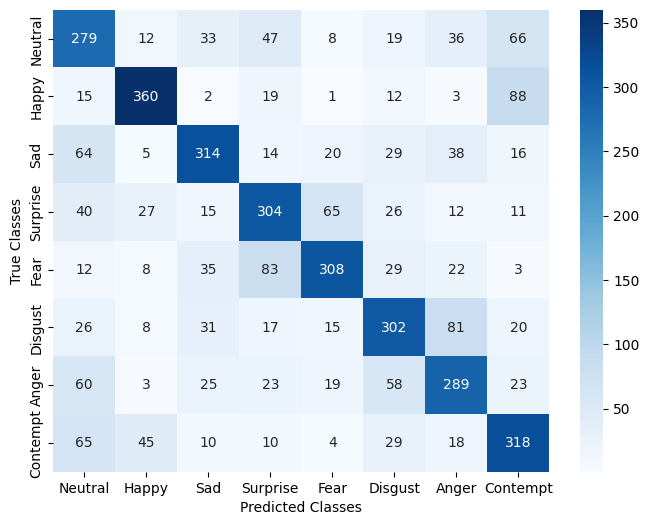
\includegraphics[width = 0.9\columnwidth]{pictures/confusion_8VA.png}
    \caption{Confusion matrix for MaxViT$_{combined}$ on AffectNet-8.}
    \label{fig:confusion_matrix_classifier}
\end{figure}

Figure \ref{fig:confusion_matrix_classifier} displays the confusion matrix of the MaxViT$_{combined}$ for \affectnet{}-8. In accordance with the theory of the circumplex model of affect, the displayed transition of discrete emotional expressions is smooth. For example, \textit{surprise} and \textit{fear} have a similar median \aro{} value or \textit{disgust} and \textit{anger} around their corresponding \val{} value. A model using continuous values can thus potentially outperform the one with discrete values. %This led us to the evaluation of the regression performance. 

\subsection{Best \affectnet{} Model Regarding Valence and Arousal}
  
In contrast to the proposed combined training methodology, the best regression results were gained with the MaxViT$_{valence-arousal}$ model. To reduce noticeable oscillating behavior during training, we reduced the training dataset by balancing according to the discrete expression labels. Furthermore, we added the CCC loss to the L$_{valence-arousal}$ loss function and used the pre-trained weights of the best model from the combined method (MaxViT$_{combined}$). With a duration of two minutes per epoch, the best results were achieved in epoch seven. 


\begin{table}[htbp]
\centering
\begin{tabular}{r | c | c | c}
\hline
\textbf{Metric} & \textbf{VGG-F}~\cite{bulat2022pretraining} & \textbf{Ours} & \textbf{Improvement} \\ 
\hline
RMSE$_{valence}$ $\downarrow$& 0.356 & \textbf{0.331} & 7,0\%\\
RMSE$_{arousal}$ $\downarrow$& 0.326 & \textbf{0.305} & 6,4\%\\
CCC$_{valence}$ $\uparrow$& 0.710 & \textbf{0.716} & 0,8\%\\
CCC$_{arousal}$ $\uparrow$& 0.629 & \textbf{0.642} & 2,0\%\\
\hline
\end{tabular}
\caption{Benchmark  vs. MaxViT$_{combined}$ for AffectNet-8}
\label{tab:benchmarkourapproach}
\end{table}

Figure~\ref{fig:affectnet_cdf} shows the percentage of data points within the absolute error range. When focusing on the ordinate, 80\% of the \va{} predictions differ only $\pm  0.3$ from their true value. The resulting model is thus more robust. %As a result, we are convinced that the learning approach led our training approach to a far robust model.

\begin{figure}[t]
    \centering
    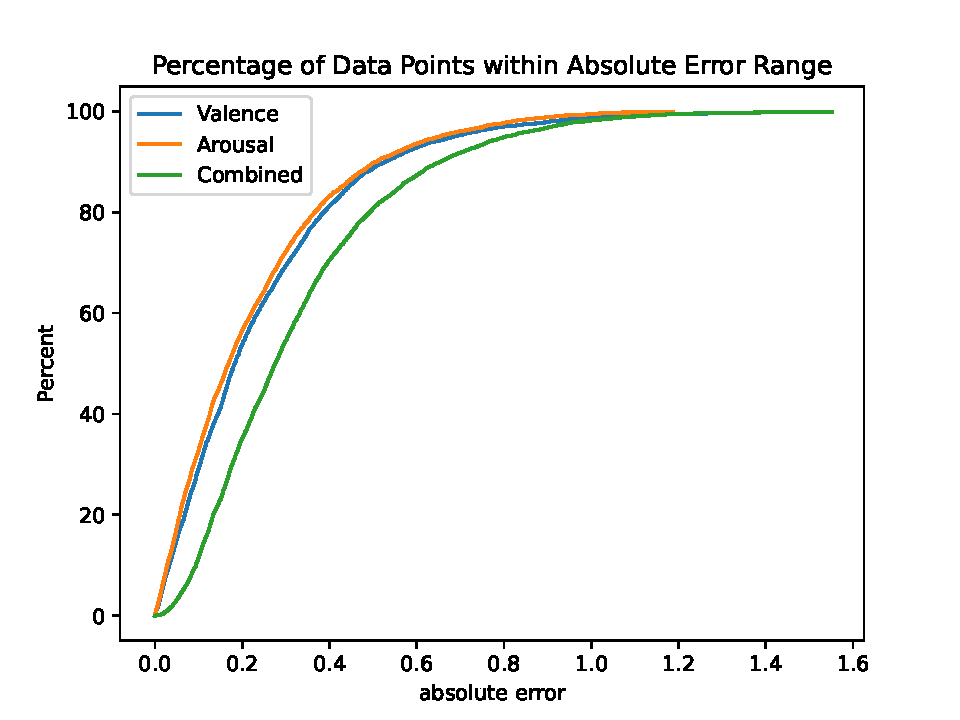
\includegraphics[width=0.95\columnwidth]{pictures/affectnet/inference_best_va_affectnet8.pdf}
    \caption{Absolute error for MaxViT$_{combined}$ trained on \affectnet{}-8.}
    \label{fig:affectnet_cdf}
\end{figure}


%\vspace{0.2cm}
\subsection{Performance of the \emotic{} Model}
 
For the \emotic{} dataset, we calculated the positive weights for each label for the training and validation dataset. Similar to the weights of the cross-entropy loss, the positive weight for each class is the inverse of the overall occurrence of a label. We chose this method to compensate for the imbalance of the frequency of expression (see Figure~\ref{fig:emotic_labeldistr}). 

 Table ~\ref{tab:benchmarkourapproachemotic} shows the overall metrics of our best EMOTIC model. To compare the RMSE of \va{} with the AffectNet dataset, we added a scaled version. For this, integers between 1 and 10 from EMOTIC are scaled to real values between -1 and 1. By definition, the CCC is invariant to shifts and scale transformations. Additionally, our EMOTIC model outperforms the best model by Khan \etal ~\cite{khan2024focusclip} according to Top-3 accuracy, which reaches 13.73 \% on the benchmark ~\cite{paperswithcodeemotop3}. 

\begin{table}[htbp]
\centering
\begin{tabular}{r | c | c}
\hline
\textbf{Metric} & \textbf{Ours} (Original) & \textbf{Ours} (Scaled) \\
\hline
Top-3 Accuracy & 14.73 \% & / \\ 
RMSE$_{valence}$ $\downarrow$& 1.150 & \textbf{0.256} \\ 
RMSE$_{arousal}$ $\downarrow$& 1.209 & \textbf{0.269}\\ 
RMSE$_{dominance}$ $\downarrow$& 1.169 & \textbf{0.260} \\ 
CCC$_{valence}$ $\uparrow$& 0.316 & \textbf{0.316} \\ 
CCC$_{arousal}$ $\uparrow$& 0.594 & \textbf{0.595} \\
CCC$_{dominance}$ $\uparrow$& 0.300 & \textbf{0.301}\\ \hline
\end{tabular}
\caption{Performance of MaxViT$_{combined}$ on EMOTIC.}
\label{tab:benchmarkourapproachemotic}
\end{table}

%Similar to our \affectnet{} model, we assessed the CDF performance of our model trained on the \emotic{} data. As shown in Figure~\ref{fig:emotic_cdf} our \emotic{} model generates similar results when assessing the body images of the test dataset. 
\subsection{Cross-Validation of the Models for Valence }

We assess the performance of the proposed trained \affectnet{}/\emotic{} model on the respective test datasets. The analysis of cross-validation results revealed that \affectnet{} outperformed \emotic{} notably in terms of absolute error metrics when evaluated on the \affectnet{} dataset. 

%\begin{figure}[t]
   %\centering
    %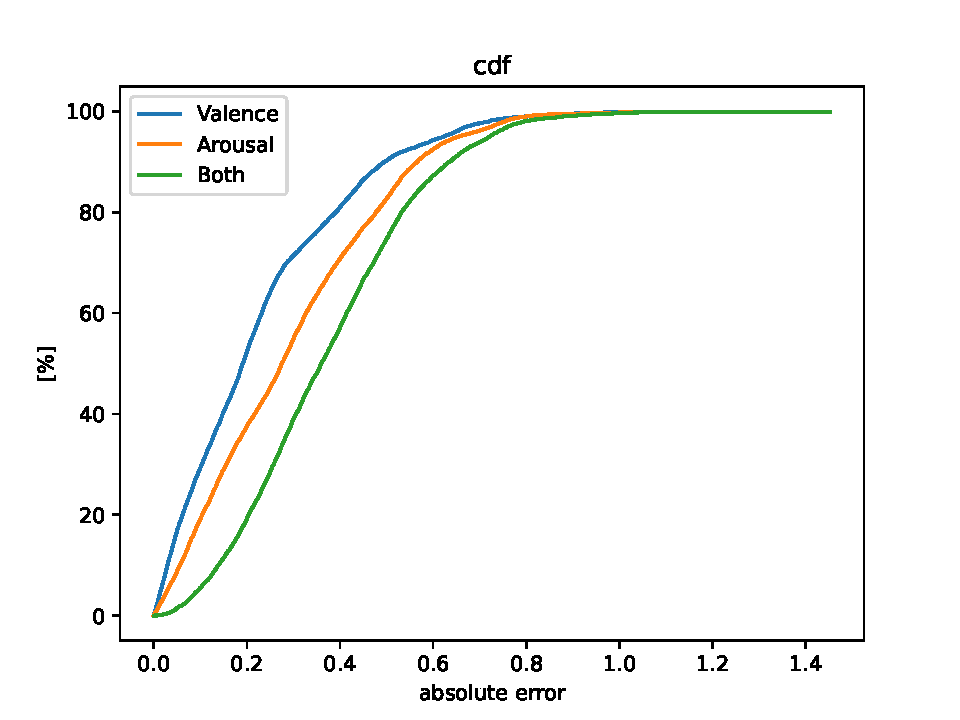
\includegraphics[width = \columnwidth]{pictures/inference_affectnet8_on_emotic.pdf}
    %\caption{CDF Absolute Error \affectnet{}-8 Model On \emotic{}}
    %\label{fig:affectnet8onemotic}
%\end{figure}

%\begin{figure}[t]
 %   \centering
  %  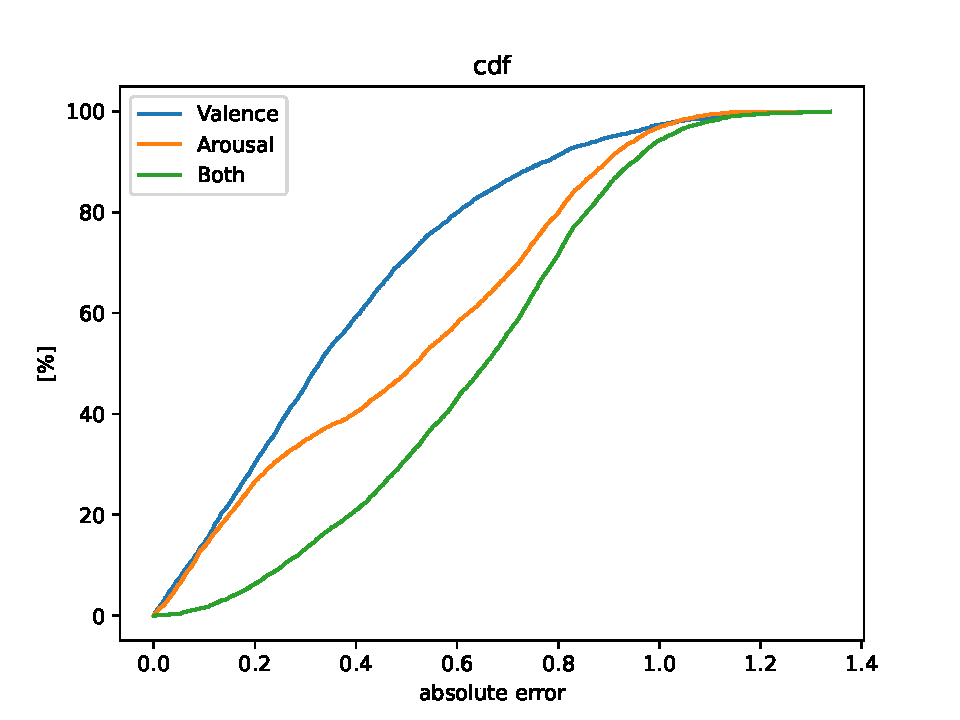
\includegraphics[width = \columnwidth]{pictures/inference_emotic_on_affectnet8.pdf}
   % \caption{CDF Absolute Error \emotic{} Model On \affectnet{}-8}
    %\label{fig:emoticonaffectnet8}
%\end{figure}

%\begin{table}[htbp]
%\centering
%\begin{tabular}{l | c | c }
%\textbf{Metric} & \textbf{\affectnet{} model} & \textbf{\emotic{} model} \\ 
%& \textbf{on \emotic{}} & \textbf{on \affectnet{}} \\ 
%\hline
%RMSE \val{} & 0.379 & 0.465 \\ 
%\hline
%RMSE \aro{} & 0.369 & 0.582 \\ 
%\hline
%CCC \val{} & 0.070 & 0.226 \\ 
%\hline
%CCC \aro{} & 0.056 & 0.007 \\ 
%\end{tabular}
%\caption{Cross Validation of our Best Models for \VA{} Estimation}
%\label{tab:benchmarkourapproachcrossvali}
%\end{table}

\begin{figure}[htbp]
    \centering
    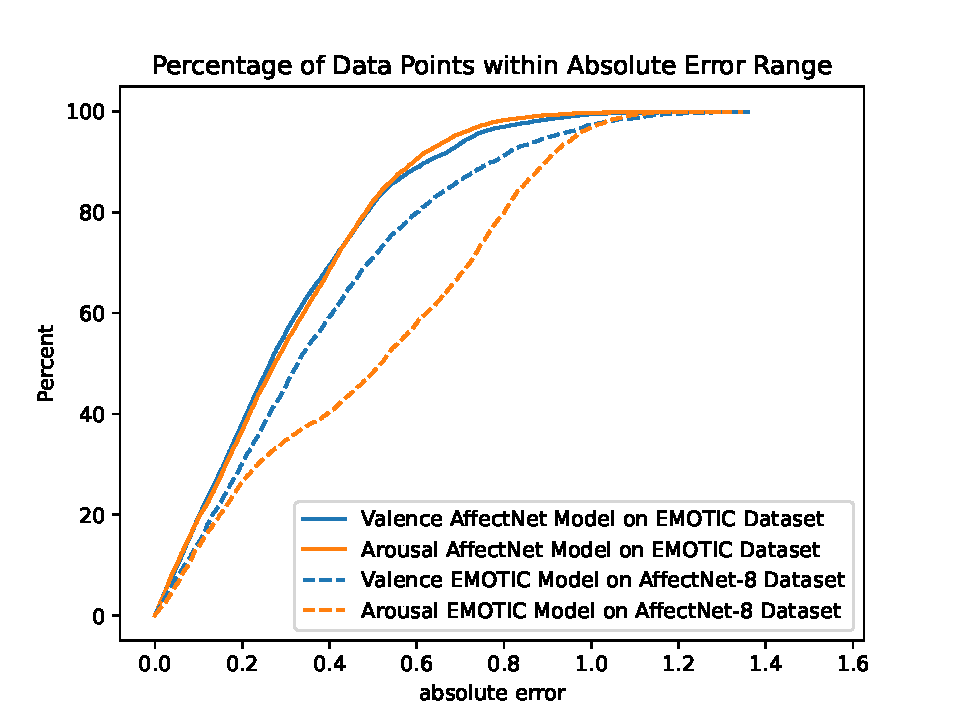
\includegraphics[width=0.95\columnwidth]{pictures/inference_cross_validation.pdf}
    \caption{Absolute error for cross-validation of the MaxViT models.}
    \label{fig:benchmarkourapproachcrossvali}
\end{figure}

As Figure \ref{fig:benchmarkourapproachcrossvali} shows, the absolute errors for \va{} are significantly higher. Thus, the substantial advantage of \affectnet{} over \emotic{} in absolute error rates during cross-validation stresses its generalization ability for expression inference tasks.
